\subsection{Koordinatsystem}
\label{Koordinatsystem}

Det koordinatsystem som brukar användas i Matematik 2B är tvådimensionellt och består av två reella tallinjer som är vinkelräta och möter varann i \textit{origo} där båda är $0$.

En position, eller \textit{koordinat}, i koordinatsystemet anges som $(x, y)$ där $x$ anger positionen längs den horisontella \textit{x-axeln} och $y$ anger positionen längs den vertikala \textit{y-axeln}.

Här är ett exempel på en koordinat $A = (3, 1)$ i detta koordinatsystem:

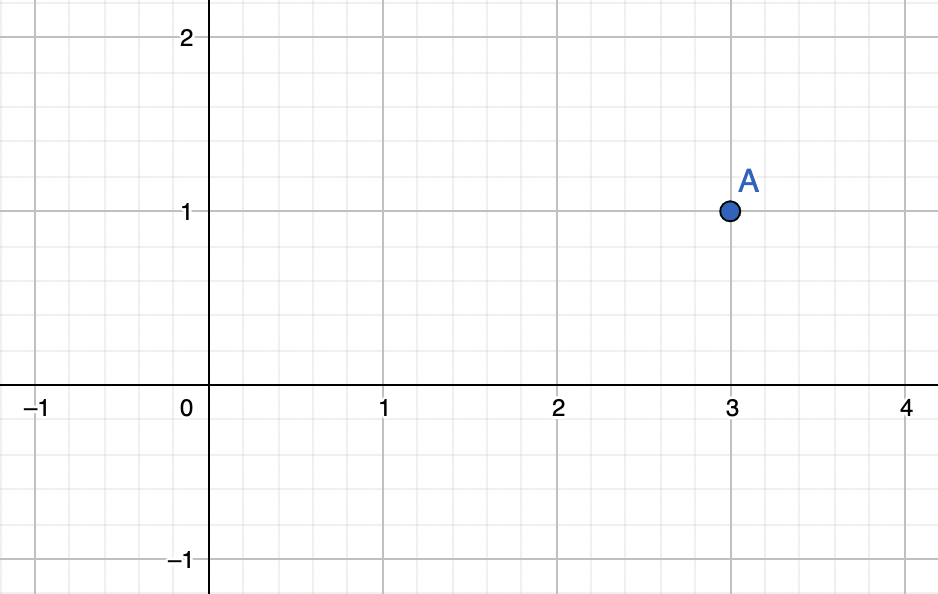
\includegraphics[width=\textwidth]{img/1.png}

\newpage
\subsubsection{Avståndsformeln}

Avståndet mellan två punkter i koordinatsystemet från \ref{Koordinatsystem} kan beräknas med hjälp av Pythagoras Sats från \ref{Pythagoras Sats}. Om vi börjar med två koordinater, $A=(2,2)$ och $B=(4,3)$

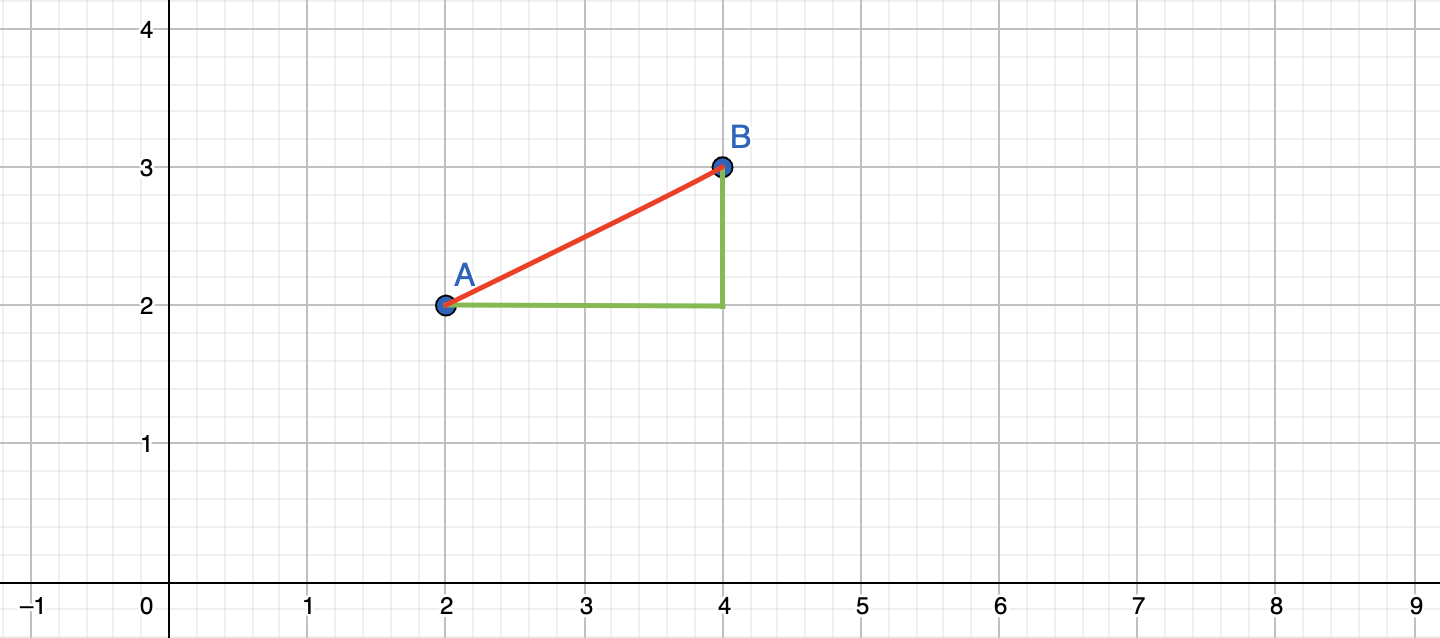
\includegraphics[width=\textwidth]{img/3.png}

Så kan vi se att de bildar en rätvinklig triangel, där en av kateterna är längs x-axeln och den andra längs y-axeln. Avståndet är då den röda linjen. Om vi vet längden av de två kateterna, så kan vi veta längden för hypotenusan, med pythagoras sats.

Längden av kateten längs x-axeln, som vi kan kalla $a$, är då absolutvärdet\footnote{absolutvärdet är distansen från $0$ på tallinjen, så t.ex är |-5| = 5. I fallet ovan så använder vi absolutvärdet då en distans aldrig kan vara negativ, men en differens mellan delar av två koordinater kan det.} av differensen mellan koordinaternas x-värden, så den kateten är

\begin{align}
	a = \\
	|2-4| = \\
	|-2| = \\
	2 \text{ (l.e)}
\end{align}

Vi kan göra exakt samma sak för kateten längs y-axeln, som vi kan kalla för $b$.

\begin{align}
	b = \\
	|2-3| = \\
	|-1| = \\
	1 \text{ (l.e)}
\end{align}

Då vi vill veta längden av hypotenusan, vilket är avståndet mellan koordinaterna, så kan vi lösa ut variabeln $c$ ur pythagoras sats, och sedan sätta in de värden vi har tagit fram.

\begin{align}
	a^2+b^2=c^2 \\
	c = \sqrt{a^2+b^2} \\
	c = \sqrt{2^2+1^2} \\
	c = \sqrt{5} \text{ (l.e)}
\end{align}

Vi kan nu generalisera det vi gjorde ovan. 

Låt $A=(a,b)$, $B=(c,d)$ och $l$  avståndet mellan koordinaterna. Då är

\begin{align}
	l = \sqrt{|a-c|^2+|b-d|^2}
\end{align}

och då absolutvärdefunktionen inte behövs, då vi ändå kvadrerar båda termerna, så kan vi förenkla detta till

\begin{align}
	l = \sqrt{(a-c)^2+(b-d)^2}.
\end{align}

\newpage
\subsubsection{Mittpunktsformeln}

Mittpunksformeln är väldigt enkel. Målet är att hitta den punkt som är mitt emellan två koordinater.

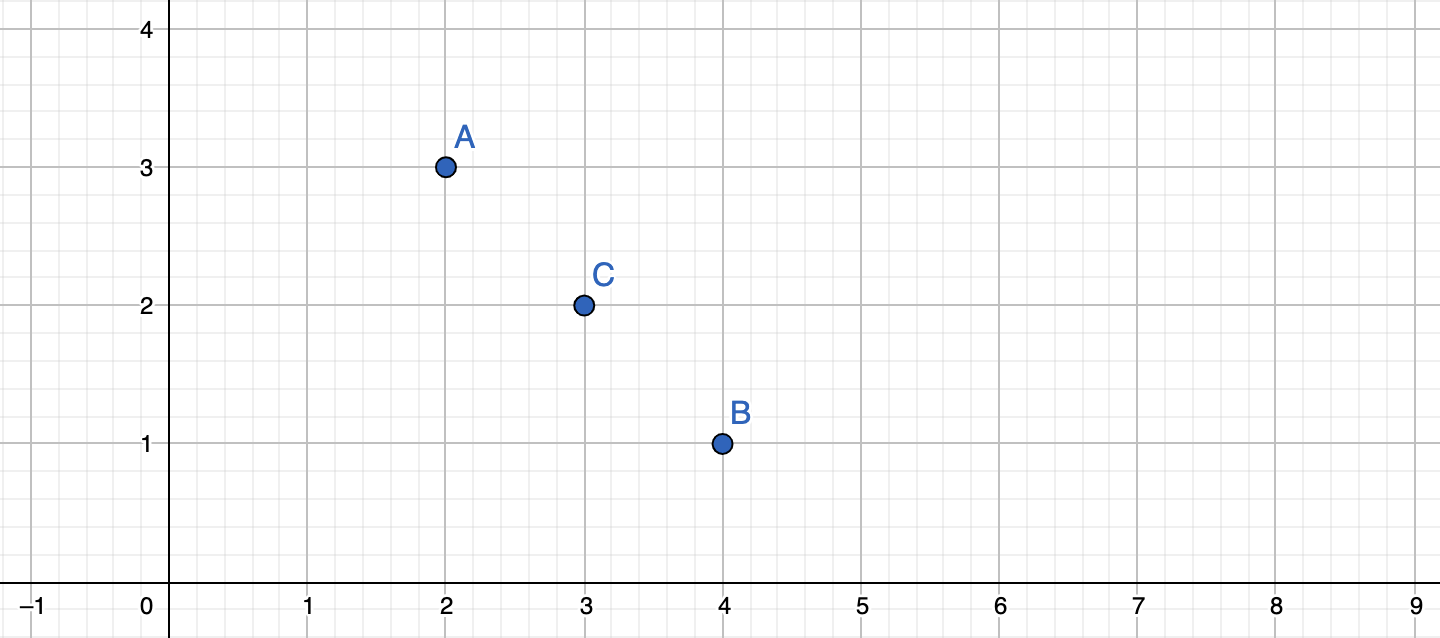
\includegraphics[width=\textwidth]{img/4.png}

Låt $A=(a,b)$, $B=(c,d)$ och låt $C$ vara deras mittpunkt. För att hitta värdet på $C$ så kan vi ta snittvärdet för $x$-värdet och sedan $y$-värdet för $A$ och $B$, vilket är $x$ och $y$-värdet för $C$, då $C$ är mitt emellan. Detta leder till att

\begin{align}
	C = \left(\frac{a+c}{2}, \frac{b+d}{2}\right)
\end{align}

\newpage
\subsection{Funktion}

En funktion inom Matematik 2B är något som översätter ett nummer till ett annat. Ett exempel är denna funktion $f$,

\begin{align}
	f(x) = \frac{1}{2}x-1
\end{align}

som översätter $2$ till $0$, eller $4$ till $1$.

vi kan rita up $f$ grafiskt i koordinatsystemet från \ref{Koordinatsystem}, genom att låta $f(x) = y$.

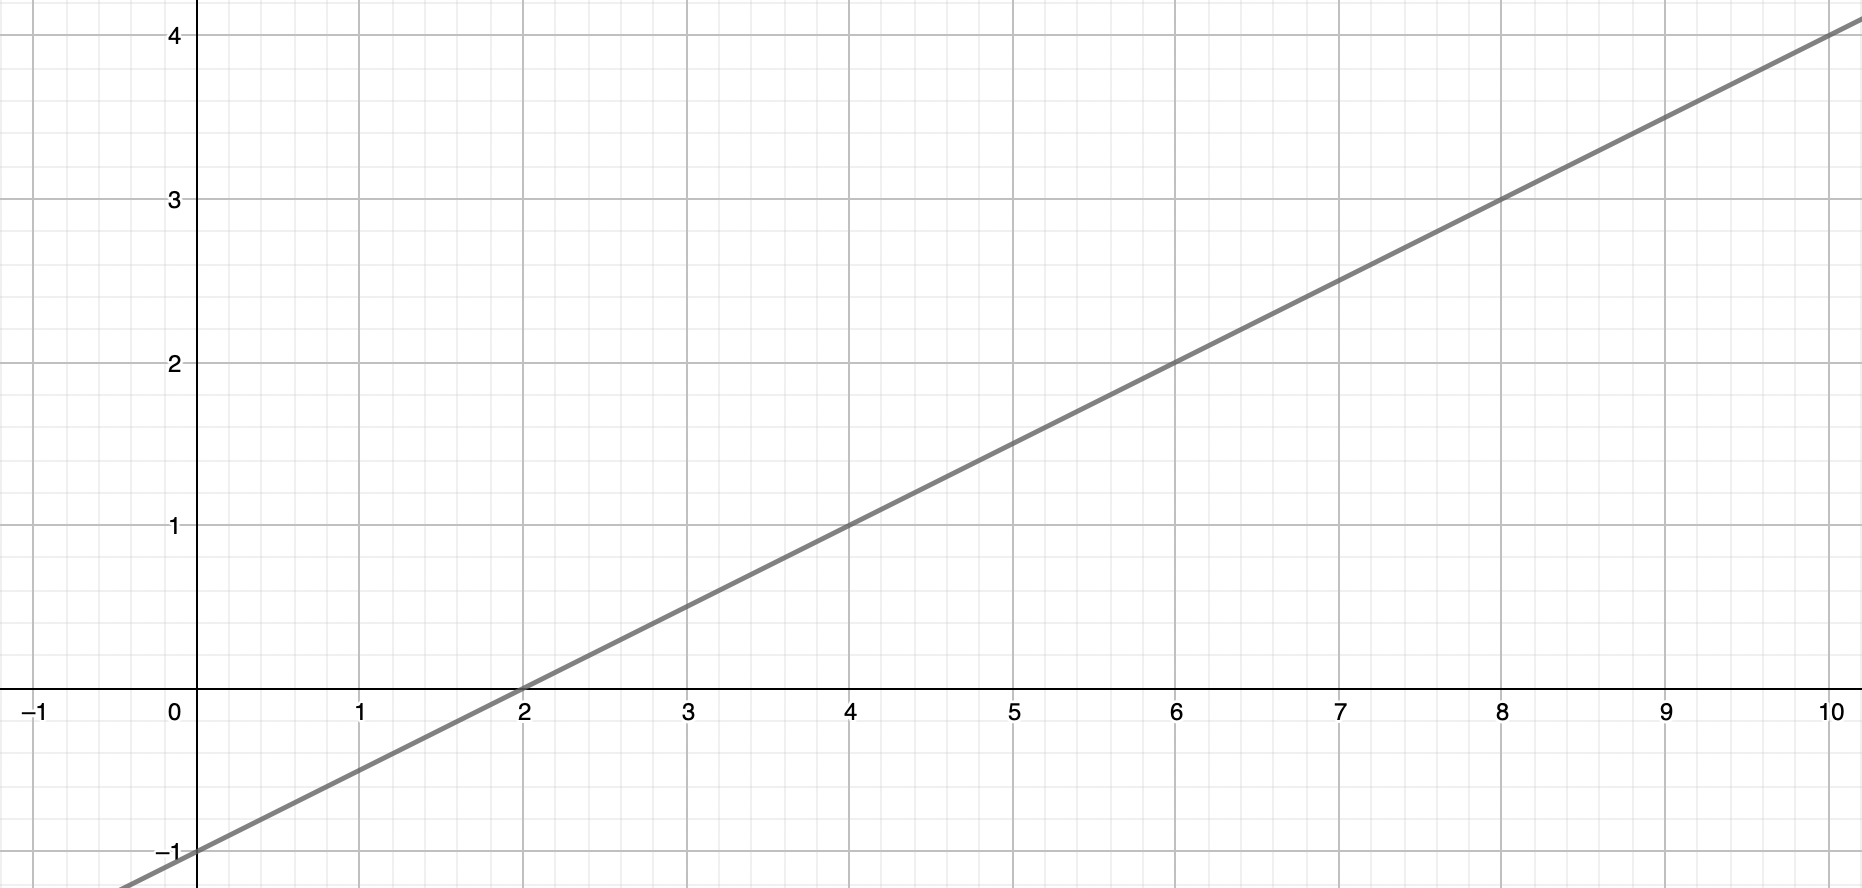
\includegraphics[width=\textwidth]{img/2.png}

\newpage
\subsection{Räta linjens ekvation}

Räta linjens ekvation brukar skrivas såhär:

\begin{align}
	y=kx+m
\end{align}

eller som en funktion:

\begin{align}
	f(x)=kx+m.
\end{align}

$k$-värdet styr förändringshastigheten, alltså hur mycket $y$-värdet förändras av en ändring hos $x$, $\frac{\Delta y}{\Delta x}$. Om $y = 3x$ så kommer $y$-värdet öka med $3$ då $x$-värdet ökar med 1. Om vi väljer två koordinater som ligger på grafen av en linjär funktion $f$, $A=(x_1,y_1)$ och $B=(x_2,y_2)$, så gäller det att

\begin{align}
	k = \frac{\Delta y}{\Delta x} = \frac{y_1-y_2}{x_1-x_2}
\end{align}

$m$-värdet styr hur mycket vi puttar upp eller puttar ner hela grafen, då det bara är en adderad konstant. $m$ värdet är också det $y$-värde där en funktion $f(x)=kx+m$ korsar $y$-axeln, då $f(0)=m$.

\begin{align}
	f(x) = kx+m \Rightarrow f(0) = m
\end{align}

\subsection{Ekvationssystem}

\subsubsection{Substitutionsmetoden}
\label{Substitutionsmetoden}

I det fallet att vi har två ekvationer, båda med samma två variabler i sig, så kan det hända att vi kan lösa fram ett värde hos vardera variabel.

Detta under kallas för ett ekvationssystem. De kan egentligen bestå av flera hundra eller mer ekvationer och variabler, men vi nöjer oss med två.

\begin{align}
	\begin{cases}
		y+2x=8 \\
		2y-x = 1
	\end{cases}
\end{align}

För att lösa det, så kan vi följa en viss stegmetod

\begin{enumerate}
	\item Lös ut en variabel ur den ena ekvationen.
	\item Ersätt variabeln i den andra ekvationen med detta uttryck och lös ekvationen.
	\item Lösningen till ekvationen sätts in i någon av de ursprungliga ekvationerna, som därefter löses.
\end{enumerate}

I fallet ovan så kan det se ut såhär:

Steg 1, jag börjar med att lösa ut en variabel ur den ena ekvationen.
\begin{align}
	y+2x = 8 \Rightarrow y = 8-2x \\
\end{align}

Steg 2, jag ersätter variabeln i den andra ekvationen med detta uttryck, så att det bara finns en variabel i ekvationen, och löser den.
\begin{align}
	2y-x = 1 \\
	2(8-2x)-x = 1 \\
	16-4x-x = 1 \\
	16-5x = 1 \\
	5x + 1 = 16 \\
	5x = 15 \\
	x = 3
\end{align}

Steg 3, jag sätter in lösningen till den andra ekvationen i den ursprungliga ekvationen, och därefter löser den med.

\begin{align}
	y+2x = 8 \\
	y+2(3) = 8 \\
	y+6 = 8 \\
	y = 2
\end{align}

Därmed är lösningen på ekvationssystemet

\begin{align*}
	x = 3 \\
	y = 2
\end{align*}

\newpage
\subsubsection{Additionsmetoden}

Additionsmetoden fungerar lite annorlunda. Istället för att lösa ut en variabel och sätta in den i en annan ekvation så multiplicerar vi hela ekvationer med konstanter och adderar in dem i andra för att eliminera variabler. Så här går det till, med samma exempel som i \ref{Substitutionsmetoden}:

\begin{align}
	\begin{cases}
		y+2x=8 \\
		2y-x = 1
	\end{cases}
\end{align}

Målet är att eliminera en variabel i varje ekvation så att vi får ekvationer med ensamma variabler i, vilket då är enkelt att lösa. Vi börjar med att multiplicera rad 1 med konstanten $(-2)$.

\begin{align}
	\begin{cases}
		-2y-4x=-16 \\
		2y-x = 1
	\end{cases}
\end{align}

Därefter kan vi addera rad 1 till rad 2

\begin{align}
	\begin{cases}
		-2y-4x=-16 \\
		-5x = -15
	\end{cases}
\end{align}

och förenkla rad 2 genom att dividera båda sidor med $(-5)$.

\begin{align}
	\begin{cases}
		-2y-4x=-16 \\
		x = 3
	\end{cases}
\end{align}

Därefter kan vi addera in rad 2, multiplicerat med konstanten $4$, i rad 1 för att eliminera $x$-variabeln där.

\begin{align}
	\begin{cases}
		-2y=-4 \\
		x = 3
	\end{cases}
\end{align}

Sedan kan vi förenkla rad 1 genom att dividera med $(-2)$ på båda sidor

\begin{align}
	\begin{cases}
		y=2 \\
		x = 3
	\end{cases}
\end{align}

Därmed har vi samma svar som i \ref{Substitutionsmetoden}, men genom en annan metod.






































